%%%%%%%%%%%%%%%%%%%%%%%%%%%%%%%%%%%%%%%%%
% Large Colored Title Article
% LaTeX Template
% Version 1.1 (25/11/12)
%
% This template has been downloaded from:
% http://www.LaTeXTemplates.com
%
% Original author:
% Frits Wenneker (http://www.howtotex.com)
%
% License:
% CC BY-NC-SA 3.0 (http://creativecommons.org/licenses/by-nc-sa/3.0/)
%
%%%%%%%%%%%%%%%%%%%%%%%%%%%%%%%%%%%%%%%%%

%----------------------------------------------------------------------------------------
%	PACKAGES AND OTHER DOCUMENT CONFIGURATIONS
%----------------------------------------------------------------------------------------

\documentclass[DIV=calc, paper=a4, fontsize=12pt]{scrartcl}	 % A4 paper and 12pt font size
\usepackage[margin=16mm]{geometry}

\usepackage{multicol}
\usepackage{sectsty} % Enables custom section titles
\usepackage{minitoc}
%\usepackage{multicol} %Enables multiple columns and additional commands
\usepackage[utf8]{inputenc}
\usepackage{lipsum} % Used for inserting dummy 'Lorem ipsum' text into the template
\usepackage[english]{babel} % English language/hyphenation
\usepackage[protrusion=true,expansion=true]{microtype} % Better typography
\usepackage{amsmath,amsfonts,amsthm} % Math packages
\usepackage[svgnames]{xcolor} % Enabling colors by their 'svgnames'
\usepackage[hang, small,labelfont=bf,up,textfont=it,up]{caption} % Custom captions under/above floats in tables or figures
\usepackage{booktabs} % Horizontal rules in tables
\usepackage{fix-cm}	 % Custom font sizes - used for the initial letter in the document
\usepackage{graphicx} %Use graphics				
\usepackage{gensymb} %More symbols

\allsectionsfont{\usefont{OT1}{phv}{b}{n}} % Change the font of all section commands

\usepackage{fancyhdr} % Needed to define custom headers/footers
\pagestyle{fancy} % Enables the custom headers/footers
\usepackage{lastpage} % Used to determine the number of pages in the document (for "Page X of Total")

\usepackage{tcolorbox}

% Headers - all currently empty
\lhead{}
\chead{}
\rhead{}

% Footers
\lfoot{}
\cfoot{}
\rfoot{\footnotesize Page \thepage\ of \pageref{LastPage}} % "Page 1 of 2"

\renewcommand{\headrulewidth}{0.0pt} % No header rule
\renewcommand{\footrulewidth}{0.4pt} % Thin footer rule

\usepackage{lettrine} % Package to accentuate the first letter of the text
\newcommand{\initial}[1]{ % Defines the command and style for the first letter
\lettrine[lines=3,lhang=0.3,nindent=0em]{
\color{DarkGoldenrod}
{\textsf{#1}}}{}}

%----------------------------------------------------------------------------------------
%	TITLE SECTION
%----------------------------------------------------------------------------------------

\usepackage{titling} % Allows custom title configuration

\newcommand{\HorRule}{\color{DarkGoldenrod} \rule{\linewidth}{1pt}} % Defines the gold horizontal rule around the title

\pretitle{\vspace{-30pt} \begin{flushleft} \HorRule \fontsize{22}{22} \usefont{OT1}{phv}{b}{n} \color{DarkRed} \selectfont} % Horizontal rule before the title

\title{Biological treasure hunting on the planet Mars} % Your article title

\posttitle{\par\end{flushleft}\vskip 0.5em} % Whitespace under the title

\preauthor{\begin{flushleft}\large \lineskip 0.5em \fontsize{12}{15} \usefont{OT1}{phv}{b}{sl} \color{DarkRed}} % Author font configuration

\author{Ingelin Garmann, Simen L. Hegge, Karsten Olav Kjensmo, Jonas Sandøy Misund, Martin Nordal, Anna Solveig Julia Testani\`{e}re, } % Your name

\postauthor{\footnotesize \usefont{OT1}{phv}{m}{sl} \color{Black} % Configuration for the institution name
Norges Tekniske og Naturvitenskaplige Universitet % Your institution

\par\end{flushleft}\HorRule} % Horizontal rule after the title

\date{} % Add a date here if you would like one to appear underneath the title block

%----------------------------------------------------------------------------------------
%	SECTION TITLE
%----------------------------------------------------------------------------------------

\sectionfont{\Large \MakeUppercase}

\subsectionfont{\normalfont \small \MakeUppercase}

%----------------------------------------------------------------------------------------
%	TEXT
%----------------------------------------------------------------------------------------

\setlength{\columnsep}{32pt}
\linespread{1.3}

%----------------------------------------------------------------------------------------

\begin{document}
\maketitle % Print the title

\thispagestyle{fancy} % Enabling the custom headers/footers for the first page 

%----------------------------------------------------------------------------------------
%	ABSTRACT
%----------------------------------------------------------------------------------------

% The first character should be within \initial{}


%----------------------------------------------------------------------------------------
%	ARTICLE CONTENTS
%----------------------------------------------------------------------------------------

\section*{Introduction}

\begin{multicols}{2}

\subsection*{What is curiosity?}
\initial{B}efore we begin, it is relevant to take a moment to fully digest the course of human history, and where we are now.
We started humble.
From our beginnings as hunter-gatherers in a nomad lifestyle with no more tools than those fashioned from stone, and no sharing of knowledge save amongst the tribal units.
Given a few thousand years, we have gone from looking at the stars with wonder to looking at the stars with determination.
The human race has reached a stage where we are capable of putting human beings into metal boxes propelled by tiny explosions and launching them out of our atmosphere.
All of this has, at some point, existed as an idea in the mind of a curious human being.
The discoveries in biology that have given us insights into how we are constructed, and the progresses of physics and engineering that have allowed us to build spacefaring crafts; all has at some point only been a figment of someone's imagination.

When the Russian cosmonauts first escaped our planet's gravity, a new realm of potential discoveries were released.
The imagination has been exposed to an embarrassment of riches since then.
The curious human mind, having discovered that the universe is vast and open to our travel, and that the unique conditions of temperature, pressure and matter that have made \textit{us}, likely exist elsewhere in the universe:

Can we reach other worlds?
What will we find there?
\textit{Are we alone?}
The thrill of discovery is immense.
Understanding history as we do, we know that a large number of years have passed, a large number of discoveries have been made, and many wise lives have come and gone and contributed to the ladder of knowledge we are currently climbing.
To fully understand our current hunt for extra-terrestrial life we need a context and to fully respect it, we must know who contributed, and how.

\end{multicols}

%------------------------------------------------

\pagebreak

\section*{The history of astronomy and biology}

\begin{multicols}{2}

\subsection{Egyptians: Astronomy as a tool for agriculture and belief}
\initial{S}ome celestial bodies like the Sun and the Moon were documented already five thousand years ago!
Indeed, astronomy being a science of observation, Egyptians did not need more than looking into the sky to discover bodies.
Although more difficult to observe, five planets could already be seen by the naked eye due to their size and brightness:
Mercury, Venus, Jupiter, Mars and Saturn.
However, we had to wait until Copernicus in 1543 to finally recognize Mars as a planet!

Egyptians' main interests for the sky were mainly agricultural and religious.
The Egyptians studied the positions and alignments of stars to build pyramids, and the size of the Moon determined periods of harvest.
For the same purpose, they already used the 365 days calendar.
Religion also played a great part in ancient astronomy as gods were viewed as constellations.
\cite{Egyptians}

\begin{center}
	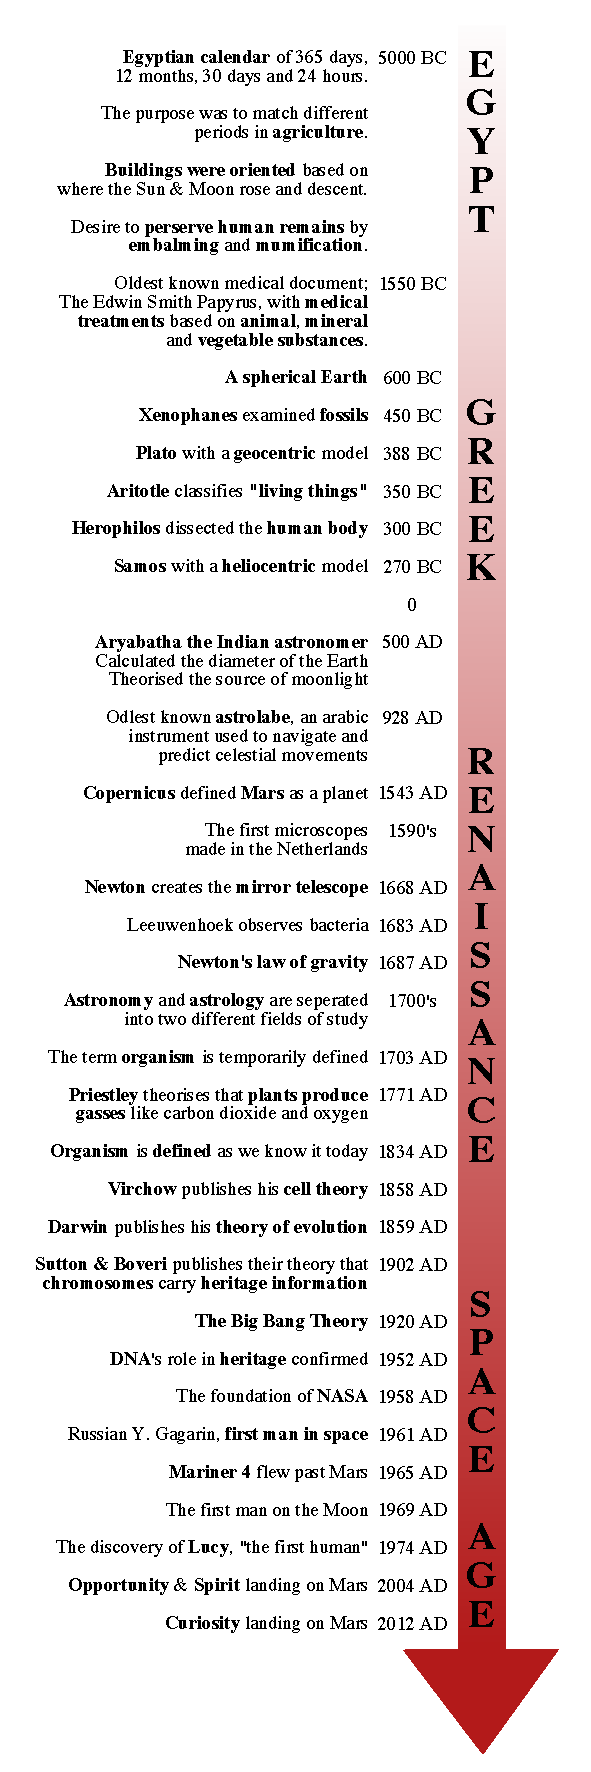
\includegraphics[width=0.475\textwidth]{timeline.pdf}
\end{center}

\subsection{Ancient Greeks, Arabs and Indians: The age of theories}
\initial{I}t is not until the Greek period, starting around 600 BC, that humanity tried to really understand and explain astronomy. 
To start with, they thought that Earth was flat, surrounded by water and that the stars were emerging from it.
Plato, followed by Ptolemy and Aristotle, were the pioneers of the geocentric model: the Sun, the Moon and the planets move in harmony around Earth, the center.

A hundred years later, another Greek, Samos, proposed the opposite theory called heliocentrism: the Sun is now the center of the Universe.
How fascinating to see how much they actually discovered at that time!  
Without tools such as the telescope, without communication within the community of scientists around the world, Greeks, Arabs and Indians still made great assumptions on how our universe worked. 
For example, the Indian astronomer, Aryabatha, not noly did he have some ideas about gravitation but also that the movement of planets around the Sun were elliptical and not circular.
He even understood that the light coming from the Moon was refracted sunlight, and not the Moon itself glowing in the dark sky.
One might wonder, how much we would know in the present time if ancient astronomers had the tools of communication we have today?
\cite{GreekAstro}
\cite{Aryabatha}

\subsection{European Renaissance: The age of reason and experimentation}
\initial{W}ith new technologies and the rediscoveries and translations of ancient Greek texts, the scientists of the renaissance period, were able to make very accurate calculations of the stars and planets.
Intellectuals in this period defined and proved the basic of astronomy as we know it today.  
Scientists such as Copernicus, Galileo and Kepler defined the heliocentric model to the world. 
It was definitely the age of reason and scientific truth. 
We can notice for example, that it is during that time that astronomy and astrology were separated into two different fields. 
Technologies and communications became more advanced and enabled physicists to search deeper and with more accuracy. 
In 1609, the Italian astronomer Galileo was one of the first people to point a telescope skyward. 
Although that telescope was far from perfected, Galileo was able to see that the Moon's surface was made of craters and mountains instead of being smooth as we thought.
As their view expanded dramatically by the telescope, astronomers were also able to discover many stars and to calculate stellar distances.
\cite{GalileoTelescope}

\subsection{Space Age: Not only studying Astronomy but also Exploring!}
\initial{I}n 1957, The Soviet Union launched Sputnik, the first spacecraft placed in orbit around Earth, marking the beginning of space exploration.
We are not only interested in studying, but also of exploring.
The space age represents an effort that is as scientific as it is political.
Indeed, this happened during the Cold War when the Soviet Union and the USA raced in different domains, including astronomy.

This space race focused particularly on discovery by humans and machines in the solar system and the development of technology.
Rockets were one of the most obvious forms of space age technology.
The creation of NASA, followed by the Apollo program was definitely highlights of the space age.
The most famous of the Apollo aircrafts was Apollo 11, carrying commander Neil Armstrong and his fellow astronauts Michael Collins and Edwin 'Buzz' Aldrin to the Moon.
On that mission, Armstrong and Aldrin were the first humans to land and walk on the Moon.
"That's one small step for a man, one giant leap for mankind."
\cite{SpaceAge}

\begin{tcolorbox}[colback=green!5,colframe=green!40!black,title=The wow! signal: Our first Extra-Terrestrial communication ? ]

On a night in 1977, Jerry Ehman, working for SETI (Search for Extra-Terrestrial Intelligence) took part in one of the world's biggest mysteries: The Wow! signal.

He was working on radio frequencies used as signals. The system is simple:\\

We measure intensity of radio frequencies. The intensity goes from 0 (the lowest) to 35 (the highest).  The intensity of the signal is normally between 0 and 2. But for 72 seconds he got an extraordinary signal: 6EQUJ5 from non-solar origin. A signal that was at its highest (the letter U) 30 times greater than the ordinary deep space noise! Amazed, Ehman wrote on the side: "Wow!", which simply became the name of the signal. But despite different theories and research on this signal, we still have no clue on what happened that night in 1977... \\

\textbf{What is 6EQUJ5?} \\

The intensity is measured between 0 and 35. Instead of just using numbers we changed 0 into a space and each numbers after 9 with the corresponding letter of the English alphabet. For example Q= 26 and U=30 

%------------------------------------------------

\section*{Physics crash course}

\subsection*{Entropy}
Imagine a room full of balls bouncing off the walls and each other.
Your image is probably a chaotic mess of balls traveling in all directions and speeds.
The order, or disorder, of the balls is what physicists call entropy.

Entropy is derived from thermodynamics, and it explains some of the most fundamental laws of our universe.

To understand what entropy really means, imagine all of the bouncing balls in your room being in the same corner at the same time.
This must be a very unlikely occurrence.
There are few ways to place all of the balls together in one corner, but lots of ways to spread them all around the room.
When all the balls are in the corner, the room has a low entropy.
If the balls are all over the place, the entropy is high.


The second law of thermodynamics says that the entropy in a closed system never decrease.
In other words; no matter what happens in a closed system, for example a room with no interaction with the outside world, there will be more and more chaos over time.
The system, or room, will eventually reach what we call a thermodynamic equilibrium.
If you want to keep the order in you room, you will need to supply it with energy.
That is partially why humans needs to eat.
Our cells use energy in chemical reactions, and we need to keep the entropy low in order for these chemical reactions to continue.
That is living beings has to be able to work against an increase in entropy, and also the reason this is one of the requirements we use to define life as we know it.

\subsection*{Spectroscopy, radiation and nuclear physics}








Spectroscopy is a method used in experimental physics to obtain information about a material.
In general one sends some kind of radiation towards the material, and then observes what happens afterwards.
Common radiation used in spectroscopy is photons, alpha, beta and gamma radiation.



% Diffraction

%------------------------------------------------

\initial{T}he seemingly trivial terms life and being alive have meanings most of us think we understand.
Surprisingly, an exact definition of life does not exist.
Instead, there has been established a list of criteria we think need to be fulfilled in order to be called life.
Such a list is given in Kjetill Østgaards \textit{Exobiologi - A hitch-hikers's guide to alien life} \cite{Exoboken} and those criteria are the basis for this section.
Considered separately, and possibly also as a whole, these criteria does not exclude examples of phenomena and machines we would not consider to be alive.
The debate concerning what life really includes is therefore open to all kinds of meta discussions and creative thinking.

\subsection{Growth}
\initial{T}he first typical criterion defines life as something that grows.
Growth is here referring to physical growth as part of a life sycle, and not personal or mental growth.
For mammals, the growth cycle starts at birth as an infant, then proceeds through the stages of youth and adulthood before ending up as an elderly individual until death.
Insects proceed through stages called egg, larvae and pupae before reaching the fully developed form of adulthood.
Both these examples are undoubtedly forms of life as we know it, but examples of inorganic phenomena subject to growth are also common.
The classical example is crystal growth describing the formation of strictly organized solid lattices.
Another example is the surface of Earth itself.
In plate tectonic theory \cite{tectonic}, the cycle of the Earth's crust can be explained by colliding and parting plates.
In a boundary zone where two plates move apart from each other, magma from inner Earth will erupt from the fissure as lava and form new crust.
In a collision zone a subduction will occur if one plate is forced underneath another, becoming part of the inner mantle.
This growth cycle of course spans over a much longer timescale than that of a mammal, but so does a mammals cycle compared to most insects.
Obviously this criterion alone does not describe life as we know it.

\subsection{Metabolism}
\initial{N}ext criterion will exclude both the crust and crystals as life forms.
It claims that a living organism must be able to support chemical reactions called metabolism.
This means that life must be able to generate new, complex molecules in a process called anabolism and to break down complex molecules into simpler ones in a process called catabolism.
In mammals, the result from anabolism is physical growth and muscle development from nutrients retrieved in the catabolism of food.
On the contrary, a chemical reactor will be able to maintain both destructive and productive reactions without actually being alive.

\subsection{Reproduction}
\initial{P}erhaps the most commonly known criterion is that life needs the ability to reproduce itself.
Humans and animals produce offspring, which contains a different set of genes than their parents.
This process called sexual reproduction requires the fusion of two sex cells \cite{reprod}.
Less complex forms of life can reproduce by simply dividing into two as some bacteria, by pollination as with most plants or by spore formation as with fungi and protozoa.
Such asexual reproductive processes will result in an offspring containing identical genetic information as the origin.
A virus - the odd one out - is not able to reproduce by itself and is dependent on its host cell in order to survive.
Thus a lot of people do not consider viruses to be life.
An even more extreme example is the offspring of a donkey and a horse.
The mule is a sterile animal, even so, most people would recognize a mule as a living organism regardless of this fact. 
Not to mention animals and humans that are born sterile or surgically made sterile.
Organic life does not have the monopoly on reproduction. Documents are easily reproduced in a copy machine, and biotechnologists have succeeded reproducing DNA in advanced PCR-machines.
The science of cloning is also widely developed and has succeeded in duplicating a living organism without the methods of traditional reproduction.
In other words, the criterion of reproduction would exclude a sterile cat as being alive, but may include inorganic phenomena that are possible to reproduce by itself or others.

\subsection{Evolution}
\initial{I}n 1859, Charles Darwin introduced the well known theory of evolution in a book called \emph{On the Origin of Species} \cite{Darwin}.
The basic idea of biological evolution is that all life on Earth shares a common ancestor!
As a result, all species roaming the Earth today are very distant cousins.
This means that all living species have a placement, according to their inherited characteristics, on a family tree.
A family tree is a representation of the evolutionary relationship among species.
This theory states that life has evolved based on a principle called \emph{survival of the fittest}.
This has resulted in the survival of the species, and the genes of the species, which were best adapted to their environment. 

On a computer, such an algorithm can easily be implemented.
The best known example is John Conway's \emph{Game of Life} \cite{Conway} which illustrates natural selection by defining four simple rules determining if a cell will live, die and/or reproduce.
The rules determining the future of one cell are all concerned with its neighbours and environment:
\begin{enumerate}
\item Any live cell with fewer than two live neighbours dies, as if caused by underpopulation.
\item Any live cell with two or three live neighbours lives on to the next generation.
\item Any live cell with more than three live neighbours dies, as if by overcrowding.
\item Any dead cell with exactly three live neighbours becomes a live cell, as if by reproduction.
\end{enumerate}
Applying these rules to all cells in a grid will lead to changes in the total amount of cells and their position for the next generation.
After applying the rules for a number of generations, the grid will look very different, but is in fact a direct outcome of the initial condition.
Evolution has taken place! 
There is now also a solid foundation for man-made evolution, the so called \emph{augmented human being}, which many of us already are.
The invention of eyeglasses is a trick on evolution - those with poor eyesight haven't evolved their way out of the problem, but have built themselves out of it instead.
Augmented humans are taking off in the coming century - \emph{biohackers} have already injected their eyes with chemicals from deep-sea fish to gain temporary nightvision\cite{biohack}, exoskeletons are being made that can help the paralyzed walk, and there are blueprints for nanorobots that can simulate blood cells and do what they do far more efficiently\cite{nanoblood}. 

\subsection{Motion}
\initial{T}he last criterion that is being considered is the phenomenon of motion.
All living organisms should be able to move and often as a response to different stimuli.
Mammals, fish and birds have either legs, fins or wings making them capable of moving their entire body.
The motion can be in an attempt to escape as a response to a threat, in chase for food or water in order to survive or simply just in order to transport itself somewhere.
In almost every activity a human can perform, a specific motion is required.
Plants are not able to move their entire body, but in order to efficiently trap sunlight, plants can turn their leaves towards the Sun.
A lot of non-living machines or vehicles are also able to move, and more and more can move on autopilot.
There also exist solar panels that can trace the Sun much like a plant, and robots that can walk and perform tasks much like a human.
Whereas some living things, like coral reefs, do not move at all.
If motion was the only criterion to be fulfilled, life would include a much wider spectrum of phenomena.
Expressions like \emph{"This storm seems to come to life with its motion, power and shape"} and \emph{"Tales come to life in the forest"} would all of a sudden have a literal interpretation. 


The past section presented and reflected on the criteria creating a definition of life.
Hopefully it became evident that a simple, straight forward definition is hard to formulate considering that the term \textit{life} must include, yet also, exclude so many phenomena.
Although there are tons of non-living examples on each of the presented criteria, the combination of properties concerning growth, metabolism, reproduction, evolution and motion are a valid basis for living creatures.
That means, of course, living creatures as we know them.
If these criteria also apply to extra-terrestrial life, only the future can answer.
Perhaps completely new lifeforms, extremely different from all earthly life, will be discovered.
With that in mind, it is an advantage that the definition of life is not carved in stone. 


While we struggle with finding a precise definition for life, we know a lot about what makes the life we have tick. A lot of the hullaballoo on Mars has been about finding \emph{water}, which is the lowest common denominator for all life as we know it. 

% Biology crash course

% How life could have started

\noindent
\initial{P}lanet Earth is often called the blue planet due to the dominant blue areas visible when viewing Earth from space.
The blue areas are our vast oceans covering more than 70\% \cite{WikiEarth} of the surface.
These oceans contain and support a broad spectrum of life, and are also a great influence on the Earth's climate and weather.
All species on Earth, eukaryotes and procaryotes alike, are dependent on water in order to survive.
A human can only survive for 5 days without water \cite{SurviveWater}, and even extremophiles called xerophiles, dry loving bacteria, need a tiny amount of water in order to function.
In other words, water is essential to life as we know it and therefore extremely interesting. 

\subsection{Chemical properties}
A single water molecule consists of three atoms: one oxygen atom and two hydrogen atoms.
The two hydrogen atoms are bonded covalently to the oxygen atom.
Due to two lone electron pairs on the oxygen, with their electrical pull, the overall structure of the is bent.
The lone pairs are not shared between the atoms.
Furthermore, the oxygen atom is much more electronegative than the hydrogen atoms, creating a dipole moment in the molecule.
This means that the oxygen will contain a slight, but significant negative charge while the two hydrogen atoms appear as slightly positive.
This creates the basis for the formation of an intricate network of hydrogen bonds as we know that positive and negative charges attract one another.  

So what makes water so unique?
First of all, the formation of hydrogen bonds gives water a high evaporation entalphy and therefore a large evaporation temperature.
To transform water from its liquid phase to vapor, energy must be applied bringing water to a temperature of 100\degree C.
On the other end of the scale, water will freeze at 0\degree C transforming to ice, which brings us to the second uniqueness of water.
In most cases, a solid phase will be denser than a liquid phase.
Thus the solid phase would sink to the bottom of the liquid phase. \cite{SolidWater}.
Polar bears floating on ice flakes in the Arctic are evidence that ice is not heavier than water.
This phenomenon has had a greater importance than just serving as a fleet for polar bears.
Without this property, ice would have sunk to the bottom in repeated cycles until there was no more liquid water during the cold periods in the history of Earth.
To sum up, due to chemical and physical properties, water remains liquid over a uniquely broad range of temperature.

However, the temperature is not the only thing that decides phase states in matter.
Pressure is equally important.
Therefore one can boil water at 70\degree C at the top Mount Everest (making it hard to boil an egg), while you need to heat it to 100\degree C at sea level \cite{WaterEverest}.
The diagram shows how this relationship between temperature and pressure affects the states of water.

\end{multicols}

\begin{center}
	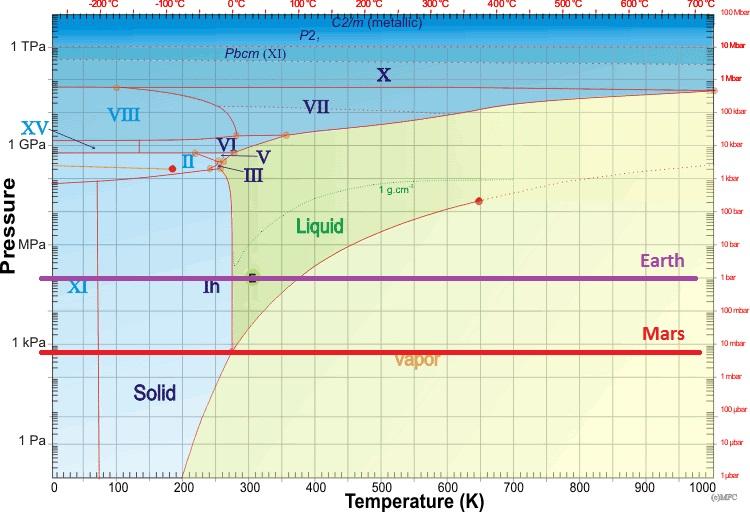
\includegraphics[width=0.9\textwidth]{water_phase_diagram_2_merka.jpg}
	% kilde: http://www1.lsbu.ac.uk/water/water_phase_diagram.html
\end{center}

\begin{multicols}{2}

Notice that although water can appear at Earth's 1 atm, which is about 101 kPa \cite{AtmEarth}, the pressure of 0,006 atm at the Martian surface \cite{AtmMars} does not allow water to be liquid.
An attempt to melt ice on Mars will result in sublimation.
The mean temperature on Earth is 15\degree C \cite{WikiEarth}.
This along with the pressure of 1 atm it makes Earth a perfect place for liquid water. 
So far, we have established that we have a lot of water on Earth, and it occurs mostly in its liquid form.
The question remaining is: what is so important with liquid water?

Liquid water has functions as both a solvent and a transport medium.
Both organic and inorganic compounds can be dissolved in water, making it a vital part of metabolism.
The blood stream is an essential transport network delivering oxygen and nutrients in our body.
Human blood plasma, the liquid part of the blood, consists of 92\% water \cite{Blood}.
On Earth, we have yet to find an organism completely independent of water. 
In fact, in all three theories concerning the origin of life, water was given a leading role as a solution bringing the organic molecules together.
As we want to find life, it seems appropriate to base our search on water.
NASAs guiding policy reflects this: \textit{Follow the water} \cite{NASAwater}. 
Water is not a rare molecule in space, in fact oxygen and hydrogen are some of the most abundant atoms in the universe.
The only problem is that the water in space most often is in the solid form of ice, and in rare occasions in form of gas.
There have been discoveries of water on Mars. 
Both poles have ice caps containing solid water \cite{MARSwater}.
Unfortunately, solid water does not have the same solvating and lubricating properties as liquid water, and will therefore not support molecular processes essential for life.
However, dry channels and craters probably formed by erosion suggest that liquid water (or some other liquid) once was present on Mars.
The best signs of life in space is therefore the discoveries of molecules we know can only be formed in contact with water.
For example, in 2002, Mars 2001 Odyssey, which is orbitting Mars, found the spectral signature of hematite, a molecule formed in water.
This mineral was later discovered by Opportunity, one of the two twin rovers exploring Mars from 2004 to 2010.
Furthermore, in 2005, Spirit, the other twin, found high concentrations of carbonate which originates in wet, near-neutral conditions. 
Carbonate actually dissolves in acid, which means that the water on this area could not have been acidic.
The rover roaming the surface of Mars today, named Curiosity, continues seeking for evidence of water. 
Where there is liquid water, there might be alien life.

(!!!no latex formatting yet!!!)

Mars: 10 facts about the red planet

Location: Mars is the 4th planet from the Sun and is the second smallest.
Size: About half the diameter of the Earth. A 100kg person would weight 38kg on Mars.
Magnetism: It has no spinning iron core and thus no planet-wide magnetic field.
Orbit: The distance from the Sun due to the elliptical orbit varies significantly more than on Earth.
Time: A year lasts for 687 Earth days. Martian day = sol = 24 hours, 39 minutes and 35 seconds.
Atmosphere: The atmosphere mainly consists of carbon dioxide (95,3%), nitrogen (2,7%) and argon (1,6%). Atmosphere on Earth has 100 times the pressure than on Mars.
Climate: Temperatures varies from -128C to 27C with an average of -53C.
Geography: Olympus Mons, the tallest known mountain, is 26km, which is approximately 3 times as tall as Mount Everest. Valles Marineris is the solar systems' largest and deepest known system of valleys.
Moons: Mars has two moons: Deimos and Phobos.
Surface: The surface has minerals containing silicon, oxygen and metals. Its red colour comes from iron oxide.

\begin{tcolorbox}[colback=red!5,colframe=DarkRed!40!black,title=Curiosity: 10 facts about the rover]

\textbf{Purpose:} To investigate the climate and geology on Mars, and to find evidences for the presence of water.

\textbf{Travel:} From November 26th 2011 at Cape Canaveral Air Force to 6th August 2012 at the Gale Crater.

\textbf{Mission duration:} One Martian year, that is 98 weeks.

\textbf{Mass/size:} The mass is 900kg. The dimensions are 3m x 2,8m x 2,1m, about the size of a car.

\textbf{Movement:} The rover can travel by an average of 30m per hour.

\textbf{Instruments:} It has 17 cameras, most of them are used to drive and navigate.

\textbf{Energy source:} The onboard nuclear power plant carries plutonium-238. From the material's decay it can produce 125W of electricity.

\textbf{Computers:} The two identical computers are specially built to tolerate the radiation that occur on Mars. They have only 256MB of RAM and 2GB of flash memory each.

\textbf{Communication:} The rover uses its three antennas to communicate in the UHF band. Direct communication to the Earth takes about 7 minutes. The rover can also communicate via Mars satellites.

\textbf{Cost:} The overall cost was 2,5 billion USD, where 1,8 billion of it was used in context of freighting the rover to Mars.

\end{tcolorbox}

% Landing the rover

%------------------------------------------------

\section*{How does Curiosity search for water?}

\subsection{ChemCam}
As one of Curiosity's tasks is to analyse the composition of the Martian surface, it carries an onboard laboratory called Chemistry & Camera (ChemCam).

The ChemCam is a composition of two separate instruments: a Laser-Induced Breakdown Spectrometer (LIBS) and a Remote Micro-Imager (RMI).

First the LIBS will use its 1067nm laser pulses to hit rocks, which small amounts of the targeted rock will reach temperatures enough for it to vaporise into plasma.
Because of the high temperature, the plasma will also emit light, telling what the rock consists of.
The emitted light will always be a seamless composition of all wave lengths, except that the presence of specific elements will leave characteristic marks where the light is gone at specific wave lengths.
These marks, typically illustrated as black stripes onto the spectrum of visible light, gives the glowing object its absorption spectrum.
The RMI is a combined microscope and camera able to focus from 1m to 7m away.
It will then measure what light the plasma has emitted, obtaining an absorption spectrum.
With the ability to distinguish between 6144 different wave lengths from 240nm to 850nm, the RMI can recognise most light elements. \cite{ChemCam}

\subsection{Curiosity's Chemistry \& Mineralogy (CheMin)}
\initial{C}uriosity is not only able to study the very surface of Mars.
With an arm attached, it can drill into the soil to excavate powdered samples from the ground.
These samples are studied with Curiosity's Chemistry \& Mineralogy (CheMin) instrument.
CheMin's main task is to conduct powder X-ray diffraction to study what minerals Martian soil consists of.
X-rays are sent through the sample powder so that these rays will create a diffraction pattern depending on each mineral component in the sample.
The diffracted rays are then captured by an X-ray sensitive 600x582 charge coupled device (CCD), that is a camera which operates with X-ray wave lengths.
The CCD may read, erase and recharge, take individual images in other words, 1000 or more times for each experiment to ensure reliable results.
Each exposure takes from 5 to 30 seconds, resulting in a 10 hour duration for each experiment. \cite{CheMin}

\subsection{Alpha Particle X-ray Spectrometer (APXS)}
\initial{T}he APXS is a spectrometer sitting on Curiosity's robot arm.
As its ancestors on the previous rovers the spectrometer is used to identify chemical elements in rock and soil on the Martian surface.
There are some differences, though.
The APXS on Curiosity is better!

\begin{center}
	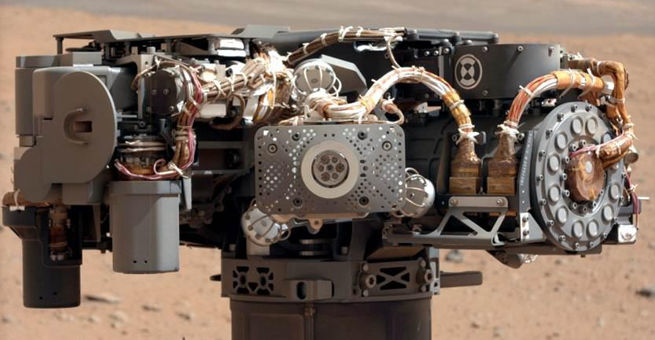
\includegraphics[width=0.475\textwidth]{curiosity_apxs.jpg}
	\tiny{Credit: NASA/JPL-Caltech/MSSS}
\end{center}

The software controlling Curiosity's arm is an improvement over the previous rovers.
This lets the arm get closer to samples on the ground while keeping the instruments safe.
In addition, the amount of radioactive material used in the source has been doubled, which increases the intensity of the ray.
Since the instruments have to operate at low temperatures, Curiosity's APXS has also been equipped with an electrical solid state cooler which lets it function during the Martian daytime.
Spirit and Opportunity could only use their APXS during night on Mars.

Most of the minerals examined contains elements like sodium, magnesium, aluminum, silicon, calcium, iron and sulfur.
APXS can also detect traces of important elements that take part in different salts: sulfur, chlorine and bromide.
These trace elements can be signs of former interactions with water.

After APXS has studied the samples, Curiosity decides if any other tests should be conducted.
The information from APXS is also used to figure out how the stone formations in the area close to the rover could have formed and changed over time.

The radioactive element curium (Cm$^{244}$) is used as a source for the alpha particles.
The element has a half life of 18.1 years, which suits this kind of long term mission.
Even after more than seven years the decrease in activity will be negligible.

The alpha particles emitted are used to excite atoms in the samples, which responds by emitting X-rays afterwards.
These X-rays will be emitted in all directions and the ones coming back towards Curiosity's robot arm can be used in spectroscopy.

Throughout history the different APXS-instruments on the rovers have given us a lot of important data.
Therefore it was brought yet again on Curiosity, and therefore research is still continuing to improve the technique and refine how we will search for water and traces of it in the future \cite{NASA-rover}.

\subsection{Dynamic Albedo of Neutrons (DAN)}
\initial{T}he Dynamic Albedo of Neutrons is an instrument on Curiosity used for the search of hydrogen in minerals or even in ice beneath the Martian surface.
However, it is unlikely that there is any ice directly beneath the surface of the Gale Crater landing site.
The instrument can detect hydrogen up to $50 cm$ below the surface, by shooting neutrons into the ground and measure how they are scattered.

The instrument is a part of the Russian contribution to Curiosity and a broad collaboration between USA and Russia.

In addition to water, DAN can be used to find suiting places to take samples for the other instruments aboard Curiosity.
The data is also complimentary with the camera images and study of the Martian surface and geology.

DAN works by aiming neutrons with high energy at the ground, and registering their energy after they have bounced back.
The loss in kinetic energy is characteristic for each element, and the amount of time it takes for the neutrons to get back, gives an indication of how much of said element is in the ground.
One of the elements that can be, and has been, detected by DAN is hydrogen.
Already before Curiosity was sent to Mars, this technology was used to find water on the red planet.
Neutrons from the background radiation in the cosmos were used as a source when the Odyssey satellite detected water back in 2002.
The hydrogen was interpreted as water close beneath the Martian surface.

DAN can also use the cosmic background radiation as a source for neutrons, but can also actively shoot neutrons towards the ground for higher resolution and more effective tests.

Hydrogen detected by DAN can be signs of former water that at the time got bound in crystals.
These crystals are called hydrated minerals, and can be left over from a wetter period on Mars.

\subsection{Radiation Assessment Detector (RAD)}
\initial{O}ne essential objective for Curiosity's mission is to study the conditions for future human journeys to Mars, of which radiation is feared to be a considerable constraint.
Curiosity carries its Radiation Assessment Detector (RAD) in order to map what kinds of radiation there are and what the levels are.
RAD points upwards in a 65 degree field-of-view to detect radiation from outer space, both particle radiation and electromagnetic waves.
In application where the purpose is to protect humans from radiation, what is also interesting is how much of the radiation that is ionizing.
Such radiation has enough energy to destroy chemical bonds, for example DNA molecules, events that in repeated occasions can lead to cancer.
RAD can for instance distinguish between such ionizing radiation and harmless radiation.
RAD has in fact been in use during the journey to Mars as well, on which a human would also have been exposed to the radiation. \cite{RAD}

% Hostile environment on Mars

% Other current space missions

%------------------------------------------------

\section*{Plans for the near future}

% Super ball bot?

% Travels to Jupiter and Europa

% Where will we search for what in the future?

% How will we search?

% What could exist out there?

%------------------------------------------------

\section*{What is life, REALLY?}

% AI

% Multiverses

% Game theory

% Simulation

\end{multicols}

%----------------------------------------------------------------------------------------
%	REFERENCE LIST
%----------------------------------------------------------------------------------------
\onecolumn
\input{"Kilder.tex"}

%----------------------------------------------------------------------------------------

\end{document}